%  Beamer slide example.

\documentclass[9pt]{beamer}
% \setbeameroption{show only notes}
%\setbeameroption{show notes}

\usepackage[utf8]{inputenc}
\usetheme{inria}
\usepackage{helvet}
\usepackage{graphicx}

\usepackage{tikz}
\usetikzlibrary{arrows,shapes,positioning,calc,shadows,trees}
\tikzset{
  mstep1/.style = {basic, rounded corners=2pt, thin, align=center, fill=orange!70,text width=1.5cm},
  mstep2/.style = {basic, rounded corners=2pt, thin, align=center, fill=green!30,text width=1.5cm},
  basic/.style  = {draw, text width=2cm, drop shadow, font=\sffamily, rectangle},
  root/.style   = {basic, rounded corners=2pt, thin, align=center,
                   fill=green!30},
  level 2/.style = {basic, rounded corners=6pt, thin,align=center, fill=green!60,
                   text width=8em},
  level 3/.style = {basic, thin, align=left, fill=pink!60, text width=6.5em}
}
\tikzstyle{every picture}+=[remember picture]
\tikzstyle{na} = [baseline=-.5ex]


\def\aboxl[#1,#2,#3,#4,#5]#6{%
  \node[draw, cylinder, alias=cyl, shape border rotate=90, aspect=#3, %
  minimum height=#1, minimum width=#2, outer sep=-0.5\pgflinewidth, %
  color=orange!40!black, left color=orange!70, right color=orange!80, middle
  color=white] (#4) at #5 {};%
  \node at #5 {#6};%
  \fill [orange!30] let \p1 = ($(cyl.before top)!0.5!(cyl.after top)$), \p2 =
  (cyl.top), \p3 = (cyl.before top), \n1={veclen(\x3-\x1,\y3-\y1)},
  \n2={veclen(\x2-\x1,\y2-\y1)} in (\p1) ellipse (\n1 and \n2); }

\author{Maurice Brémond \and Gaëtan Harter}

\title[Intégration continue]{L'Intégration Continue}
% \subtitle{Dans un contexte de développement Inria}
\subtitle{Présentation IJD}

% Automatically insert a "new section" page at each section.
\AtBeginSection[]{
  \begin{frame}[plain]
    \partpage
  \end{frame}
}
% \inriaswitchcolors COLOR
%
% Where COLOR is one of red, blue, orange, darkblue, violet,
% pastelgreen, grey, or green.
\newcommand{\inriaswitchcolors}[1]{%
  \pgfaliasimage{figfootline}{figfootline-#1}% !!!
  \pgfaliasimage{figbackground}{figbackground-#1}% !!!
  \pgfaliasimage{figbackground}{figbackground-#1}% !!!
}

% frame with toc for current subsection
\newcommand{\tocsubsection}[1]{
  \begin{frame}
    \tableofcontents[
      currentsubsection,
      sectionstyle=show/shaded,
      subsectionstyle=show/shaded,
      subsubsectionstyle=show/show/shaded
    ]
    #1
  \end{frame}
}
% starting the document
% *********************
\begin{document}

% titlepage
% ---------
\begin{frame}[plain]
  \titlepage
\end{frame}
% table of contents
% -----------------
\begin{frame}{\textcolor{inriaGrey}{Table des matières}}
  \tableofcontents
\end{frame}



% Introduction
% ************

\inriaswitchcolors{red}
\section{Quid de l'intégration continue}

\begin{frame}{Problématiques}
\begin{block}{problématiques}
  \begin{itemize}
  \item quel compilateur, quels arguments
  \item dépendances entre fichiers sources
  \item éditions de liens avec les librairies externes
  \item \dots
  \end{itemize}
\end{block}
\begin{block}{des moteurs de production}
  \begin{itemize}
  \item make
  \item autotools
  \item cmake
  \item scons
  \item qmake
  \item \dots
  \end{itemize}
\end{block}
\end{frame}

\begin{frame}{Le test}
\begin{block}{}
  \begin{itemize}
  \item analyse statique    : pep8, pylint, clang static analyzer
  \item analyse dynamique   : valgrind
  \item unitaire
  \item \dots
  \end{itemize}
\end{block}
\begin{block}{Tests unitaires des outils}
  \begin{itemize}
  \item cppunit
  \item unittest, pytest
  \item junit
  \item \dots
  \end{itemize}
\end{block}
\end{frame}


\subsection{Qu'est-ce que c'est}
\begin{frame}{}
\begin{block}{Intégration}
  \begin{itemize}
  \item mise en oeuvre de la chaine de test et de production d'un logiciel
  \end{itemize}
\begin{tikzpicture}
  \node[] (developer1) {
\includegraphics[width=.04\textwidth] {images/Laptop-icon.png}};
  \node[below=.001cm of developer1] (developer2) {
\includegraphics[width=.04\textwidth] {images/Laptop-icon.png}};
  \node[below=.001cm of developer2] (developer3) {
\includegraphics[width=.04\textwidth] {images/Laptop-icon.png}};
  \node[right=1.3cm of developer2] (code_repo_db) {};
  \node[above=.4cm of code_repo_db] (code_repo_db_north) {};
  \node[left=.2cm of code_repo_db] (code_repo_db_west) {};
  \node[below=.1cm of code_repo_db] (code_repo_db_south) {};
  \node[below=.9cm of code_repo_db,mstep1] (code_repo) {gestion de versions};
  \aboxl[25,20,1.6,a1,(code_repo_db)] {};
  \node[right=.6cm of code_repo,mstep2] (build) {fabrication};
  \node[above=.4cm of build] (nux) {
\includegraphics[width=.04\textwidth] {images/Linux-icon.png}};
  \node[above=.001cm of nux] (windows) {
\includegraphics[width=.04\textwidth] {images/Windows-icon.png}};
  \node[above=.001cm of windows] (freebsd) {
\includegraphics[width=.04\textwidth] {images/Apps-freebsd-icon.png}};
  \node[right=.6cm of build,mstep2] (tests) {tests};
  \node[above=.4cm of tests] (test_ok1) {
\includegraphics[width=.02\textwidth] {images/accept-icon.png}};
  \node[above=.001cm of test_ok1] (test_ok2) {
\includegraphics[width=.02\textwidth] {images/accept-icon.png}};
  \node[above=.001cm of test_ok2] (test_bad1) {
\includegraphics[width=.02\textwidth] {images/delete-icon.png}};
  \node[above=.001cm of test_bad1] (test_ok4) {
\includegraphics[width=.02\textwidth] {images/accept-icon.png}};
  \node[right=.001cm of test_ok1] (test_bad1) {
\includegraphics[width=.02\textwidth] {images/delete-icon.png}};
  \node[right=.001cm of test_ok2] (test_ok3) {
\includegraphics[width=.02\textwidth] {images/accept-icon.png}};
  \node[right=.6cm of tests,mstep2] (install) {installation paquetage};
  \node[above=.4cm of install] (package) {
\includegraphics[width=.06\textwidth] {images/System-Package-icon.png}};
  \path[<->, thick, color=blue] (developer1) edge [bend left] (code_repo_db_north);
  \path[<->, thick, color=blue] (developer2) edge [] (code_repo_db_west);
  \path[<->, thick, color=blue] (developer3) edge [bend right] (code_repo_db_south);
  \path[->, thick, color=gray,dotted] (code_repo.east) edge [] (build.west);
  \path[->, thick, color=gray,dotted] (build) edge [] (tests);
  \path[->, thick, color=gray,dotted] (tests) edge [] (install);
\end{tikzpicture}
\end{block}
\begin{block}{en continu}
\begin{itemize}
\item à chaque nouvelle version pour les tests rapides
\item régulièrement : chaque nuit, chaque semaine pour les tests longs.
\end{itemize}
\end{block}
\begin{block}{Pourquoi ?}
  Un cycle court pour traiter au plus tôt les problèmes :
  \begin{itemize}
  \item les régressions 
  \item les codes difficiles à fusionner 
  \item cf extrem programming
  \end{itemize}

  Cela suppose d'être \textbf{actif} ! sinon c'est sans intérêt\dots

\end{block}
\end{frame}





\begin{frame}{L'automatisation}

%
%    2.1 Maintain a code repository
%    2.2 Automate the build
%    2.3 Make the build self-testing
%    2.4 Everyone commits to the baseline every day
%    2.5 Every commit (to baseline) should be built
%    2.6 Keep the build fast
%    2.7 Test in a clone of the production environment
%    2.8 Make it easy to get the latest deliverables
%    2.9 Everyone can see the results of the latest build
%    2.10 Automate deployment
%

  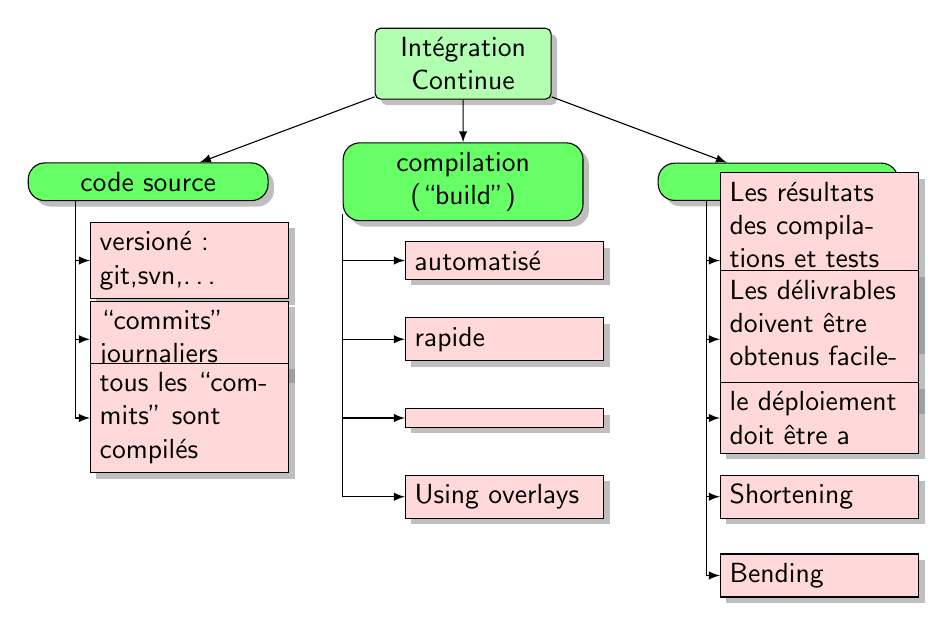
\begin{tikzpicture}[
  level 1/.style={sibling distance=40mm},
  edge from parent/.style={->,draw},
  >=latex]

% root of the the initial tree, level 1
\node[root] {Intégration Continue}
% The first level, as children of the initial tree
  child {node[level 2] (c1) {code source}}
  child {node[level 2] (c2) {compilation (``build'')}}
  child {node[level 2] (c3) {sorties}};

% The second level, relatively positioned nodes
\begin{scope}[every node/.style={level 3}]
\node [below of = c1, xshift=15pt] (c11) {versioné : git,svn,\dots};
\node [below of = c11] (c12) {``commits'' journaliers};
\node [below of = c12] (c13) {tous les ``commits'' sont compilés};

\node [below of = c2, xshift=15pt] (c21) {automatisé};
\node [below of = c21] (c22) {rapide};
\node [below of = c22] (c23) {};
\node [below of = c23] (c24) {Using overlays};

\node [below of = c3, xshift=15pt] (c31) {Les résultats des compilations et tests doivent être partagés};
\node [below of = c31] (c32) {Les délivrables doivent être obtenus facilement};
\node [below of = c32] (c33) {le déploiement doit être a};
\node [below of = c33] (c34) {Shortening};
\node [below of = c34] (c35) {Bending};
\end{scope}

% lines from each level 1 node to every one of its "children"
\foreach \value in {1,2,3}
  \draw[->] (c1.195) |- (c1\value.west);

\foreach \value in {1,...,4}
  \draw[->] (c2.195) |- (c2\value.west);

\foreach \value in {1,...,5}
  \draw[->] (c3.195) |- (c3\value.west);
    % \node [draw,rectangle,fill=gray] at (8,0) {Intégration continue}
    % child {node [draw,rectangle,fill=gray] {compilations automatiques}}
    % child {node [draw,rectangle,fill=gray] {tests automatiques}}
    % child {node [draw,rectangle,fill=gray] {``commits'' journaliers}}
    % child {node [draw,rectangle,fill=gray] {tous les ``commits'' doivent être compilés et testés}}
    % child {node [draw,rectangle,fill=gray] {la compilation doit rester rapide}}
    % child {node [draw,rectangle,fill=gray] {le test ne doit pas se faire dans l'environnement de production}}
    % child {node [draw,rectangle,fill=gray] {les résultats des dernières compilations et tests doivent être visibles}}
    % child {node [draw,rectangle,fill=gray] {le déploiement doit être automatisé}};

  
   % \node[draw,rectangle,color=black] {Intégration continue}
   % node[] {dépôt du code source \textbf{versionné}}
   % child { node[] {compilations automatiques} }
   % child { node[] {tests automatiques} }
   % child { node[] {``commits'' journaliers} }
   % child { node[] {tous les ``commits'' doivent être compilés} }
   % child { node[] {la compilation doit rester rapide} }
   %    child { node[] {le test ne doit pas se faire dans l'environnement de production} }
   %    child { node[] {le dernier délivrable doit être disponible facilement} }
   %    child { node[] {les résultats des dernières compilations et tests doivent être visibles} }
   %    child { node[] {le déploiement doit être automatisé} }
   %  } ;
  \end{tikzpicture}
    
\end{frame}



% L'intégration continue à Inria
% ******************************
\inriaswitchcolors{blue}
\section{L'intégration continue à l'Inria}

\begin{frame}{https://ci.inria.fr/}
\begin{tikzpicture}
  \node[] (root) {};
  \node[below=3.5cm of root] (root_south) {};
  \node[] (ci_main)  {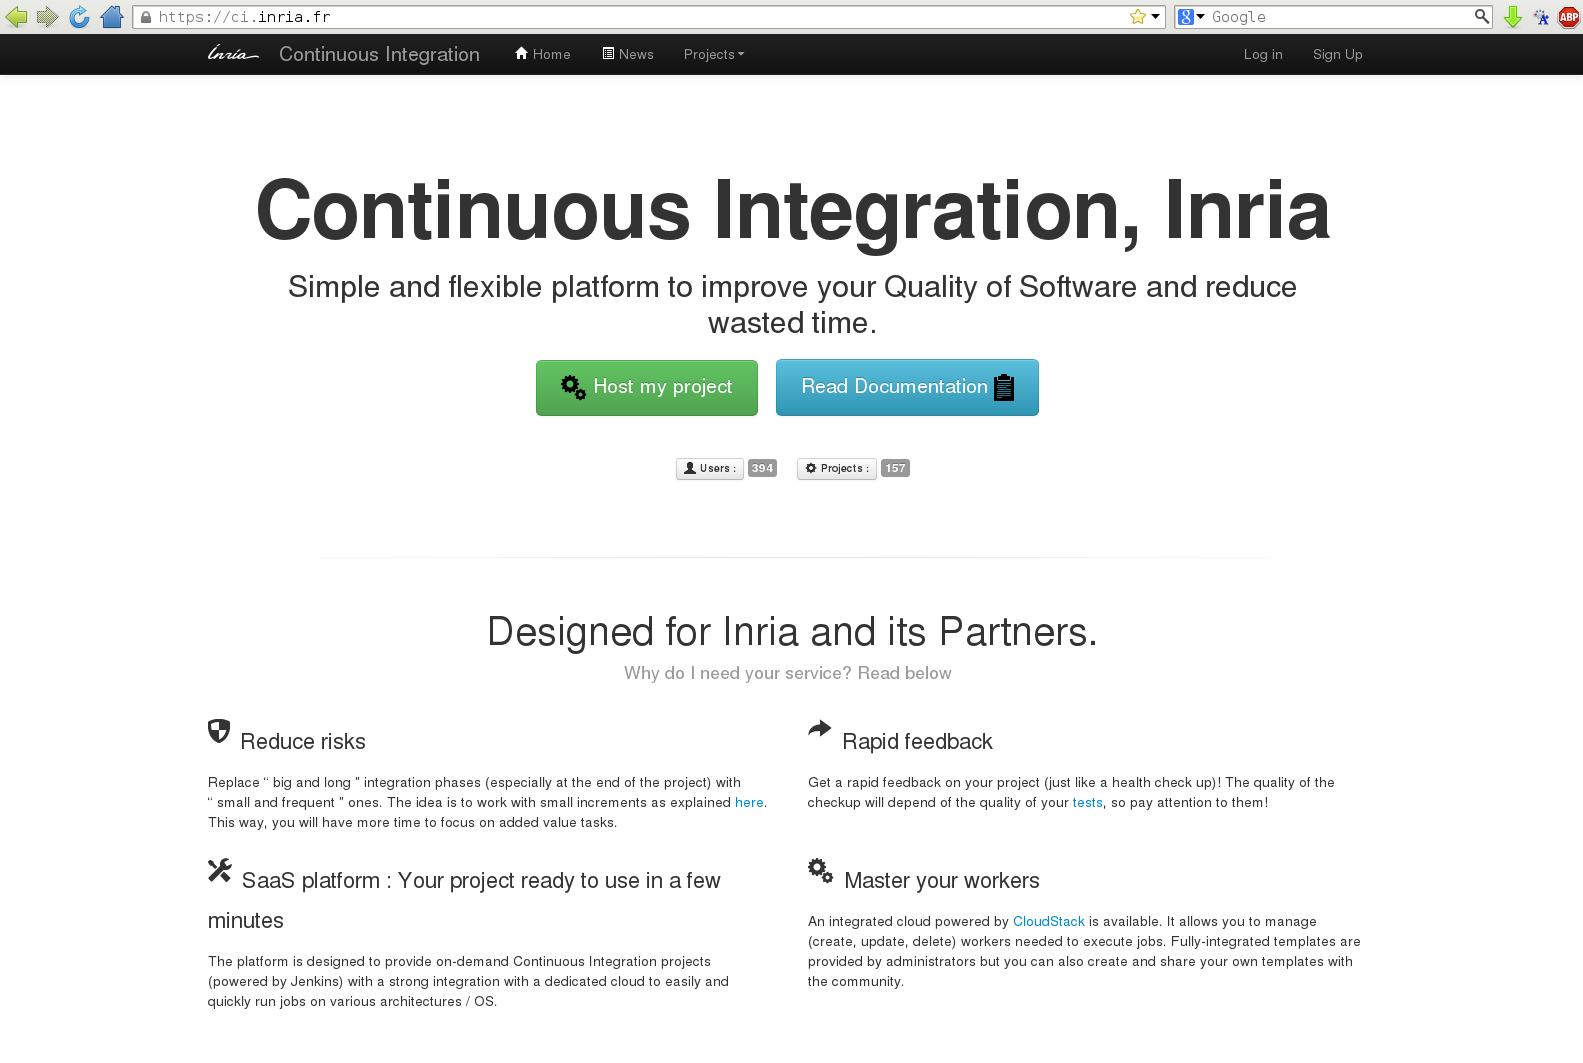
\includegraphics[width=.9\textwidth] {images/ci-main.png}};
  \node[right=1.1cm of root_south,draw,rectangle,thick,drop shadow,color=gray,rounded corners=2pt] (ci_doc)  {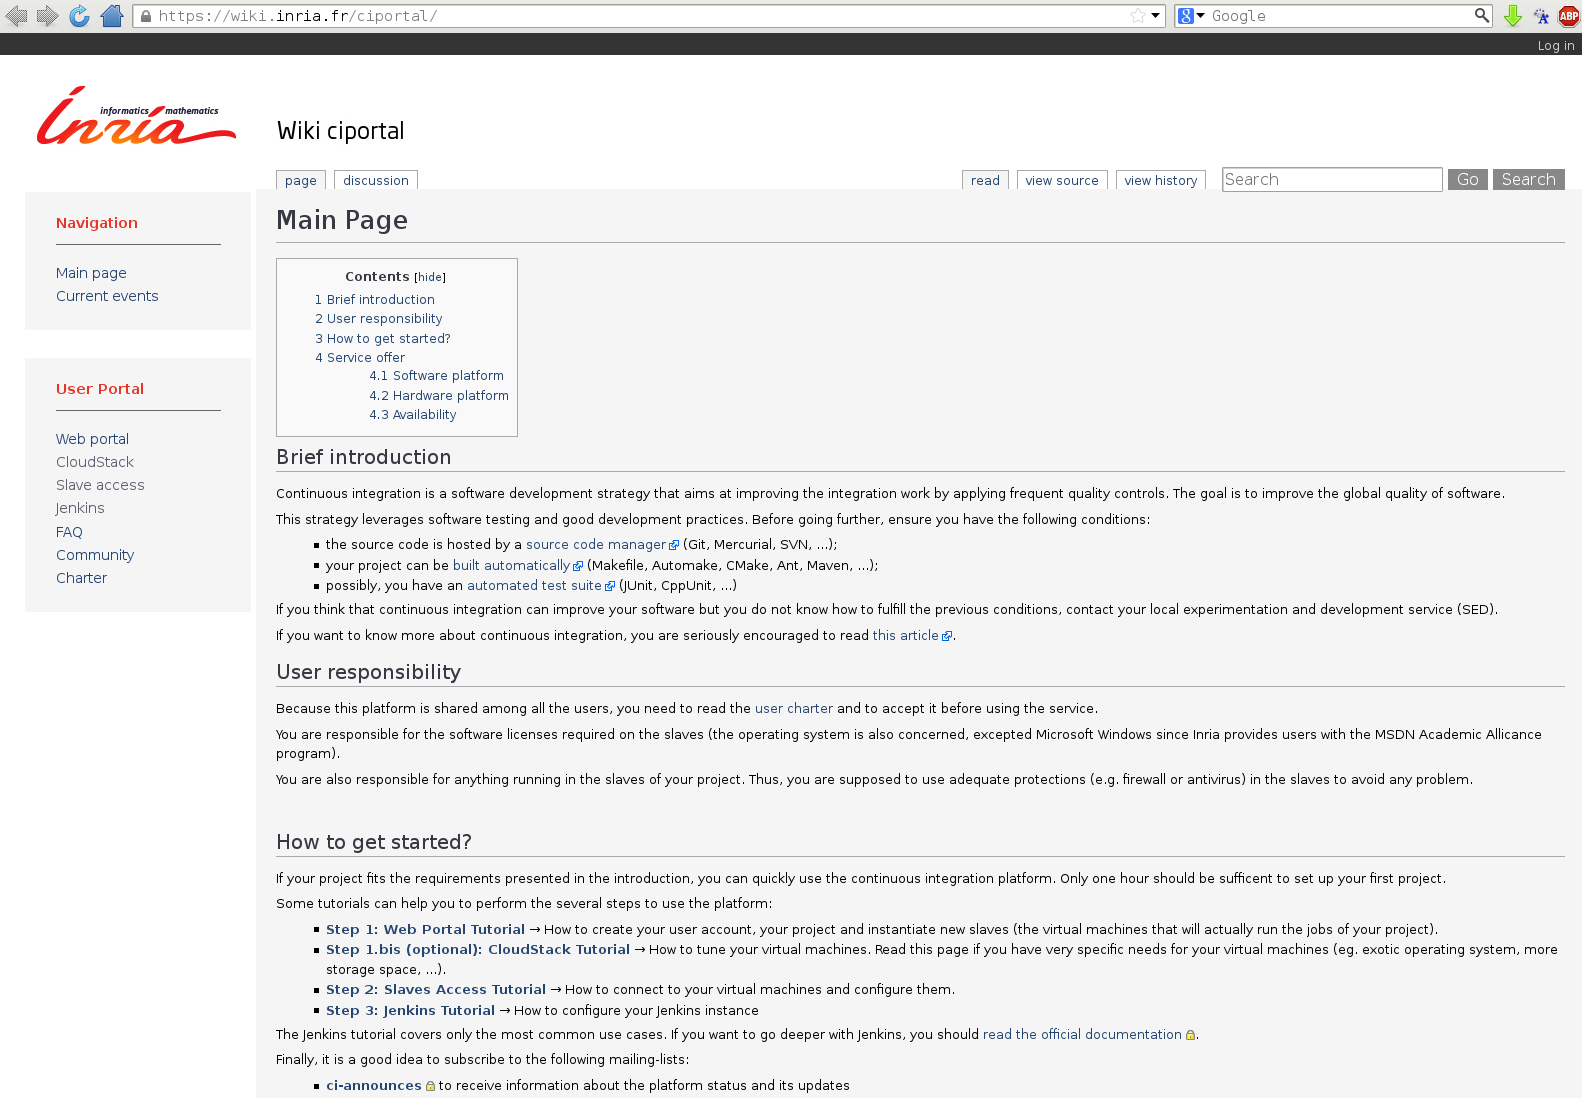
\includegraphics[width=.9\textwidth] {images/ci-doc.png}};
  \node[draw,ellipse,minimum height=.8cm,minimum width=2.5cm,thick,color=red] at (.7,0.9) (ok) {};
  \path[->, thick, color=red] (.6,.2) edge [bend right] (.9,-.2);
\end{tikzpicture}
\end{frame}

\begin{frame}{Un projet}
\begin{tikzpicture}
 \node[] (project)  {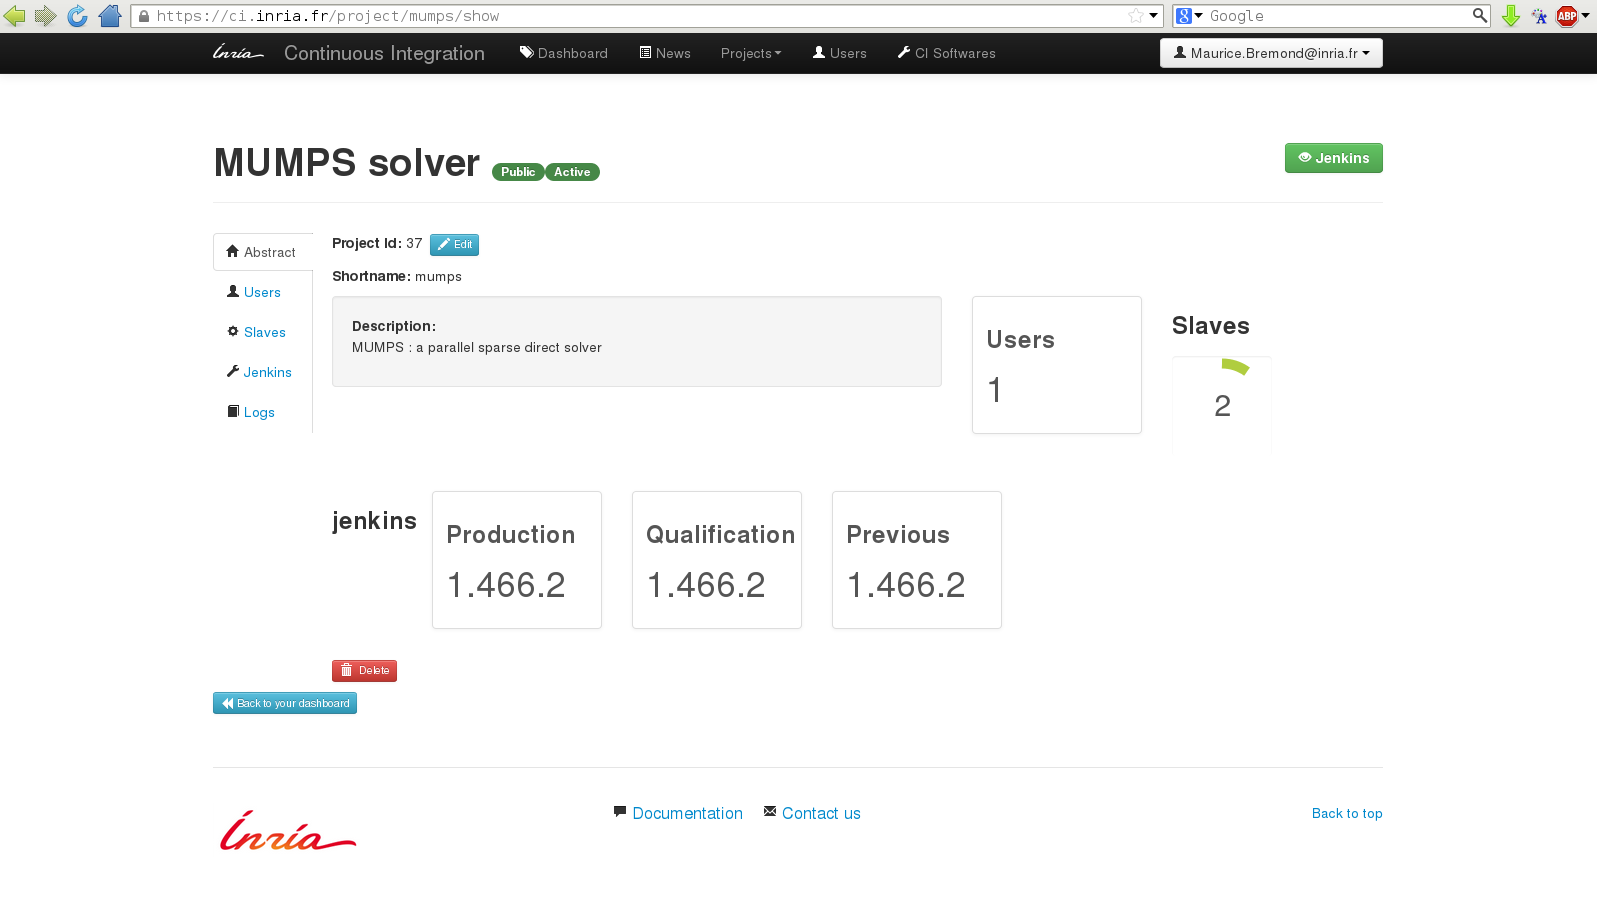
\includegraphics[width=1.2\textwidth] {images/ci-project.png}};
\end{tikzpicture}
\end{frame}

\begin{frame}{Gestion simple des machines virtuelles associées}
\begin{tikzpicture}
 \node[] (project)  {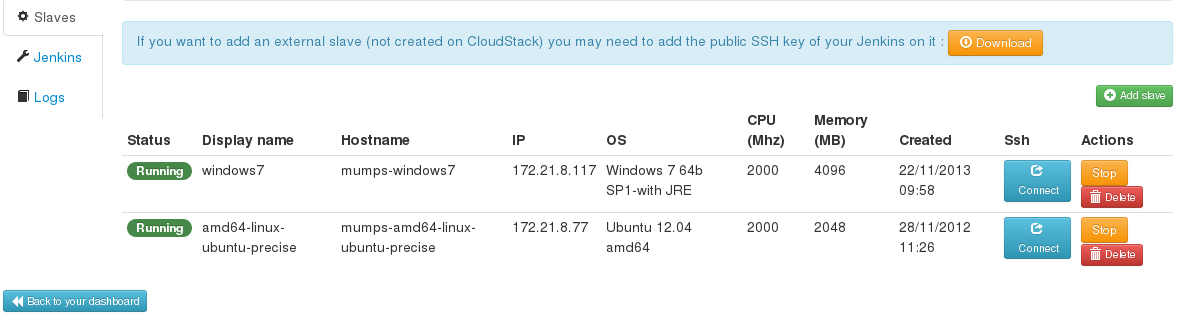
\includegraphics[width=1.2\textwidth] {images/ci-slaves.png}};
\end{tikzpicture}
\end{frame}

\begin{frame}{Création d'une nouvelle machine}
\begin{tikzpicture}
 \node[] (project)  {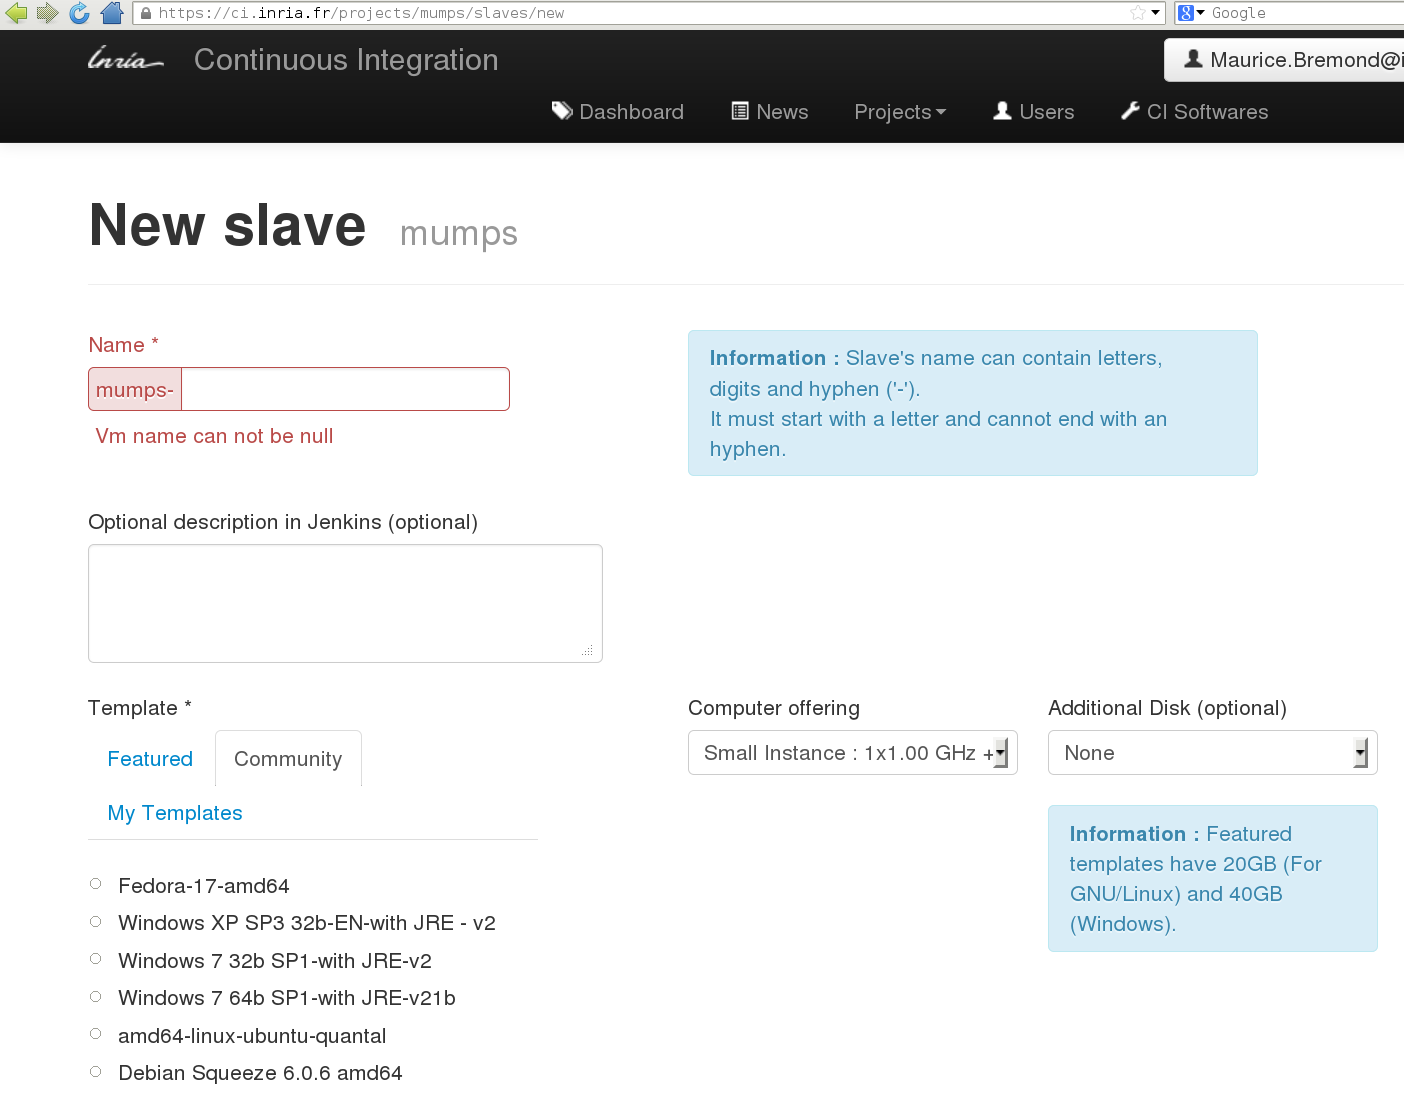
\includegraphics[width=.9\textwidth] {images/new-slave.png}};
\end{tikzpicture}
\end{frame}


\begin{frame}{Accès direct au gestionnaire sous-jacent : cloudstack}
\begin{tikzpicture}
 \node[] (project)  {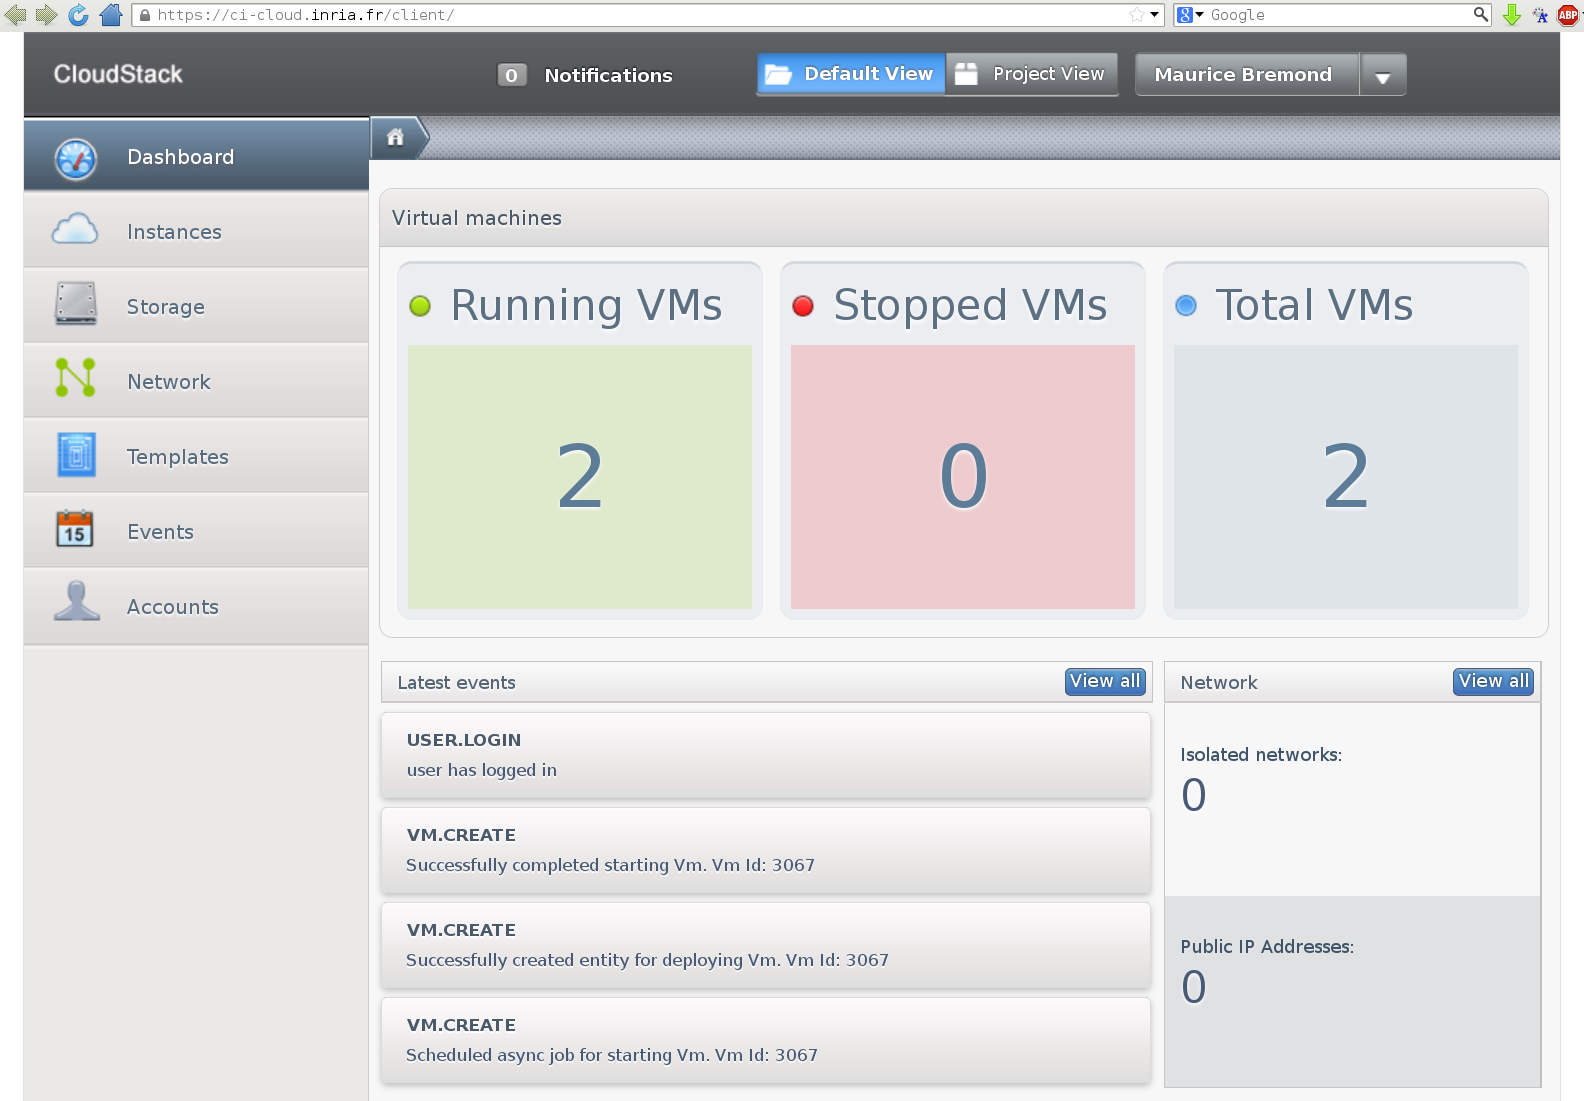
\includegraphics[width=1.2\textwidth] {images/cloudstack-main.png}};
\end{tikzpicture}
\end{frame}

\begin{frame}{Accès direct au gestionnaire sous-jacent : cloudstack/machine}
\begin{tikzpicture}
 \node[] (windows_conf)  {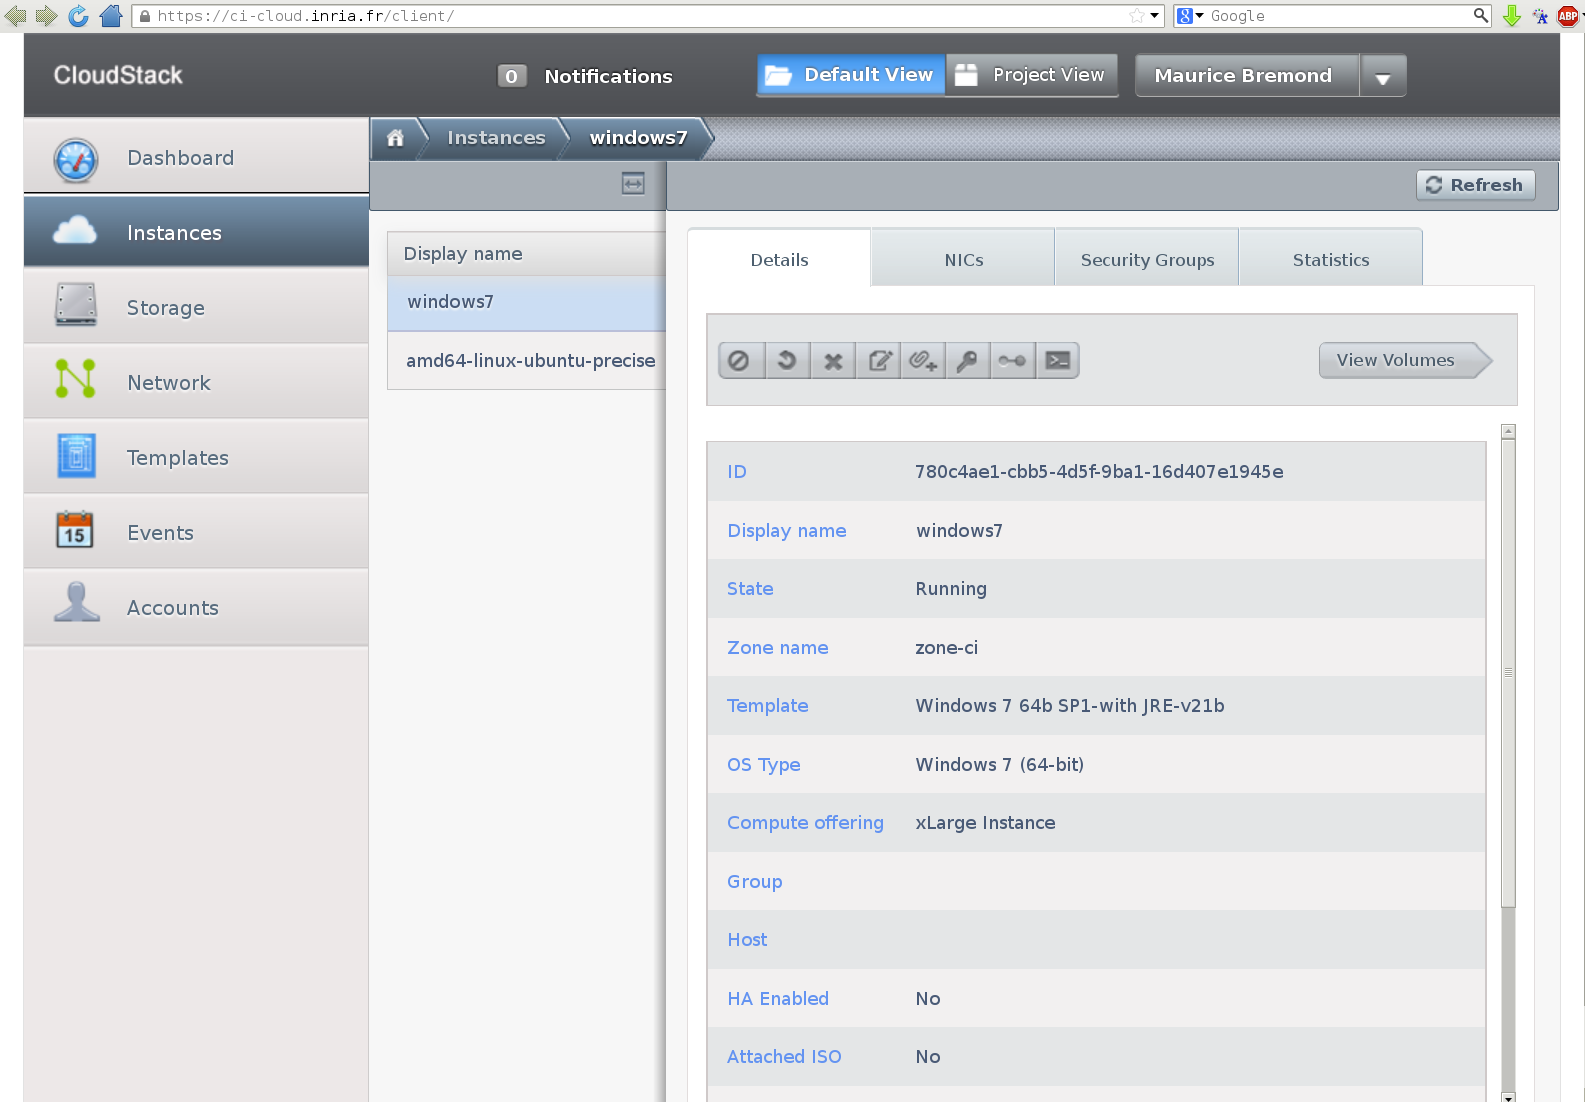
\includegraphics[width=1.2\textwidth] {images/cloudstack-windows-conf.png}};
 \node[draw,ellipse,minimum height=.8cm,minimum width=.8cm,thick,color=red] at (2.3,1.6) (select) {};
 \node[] at (-4,-0.4) (windows_desktop) {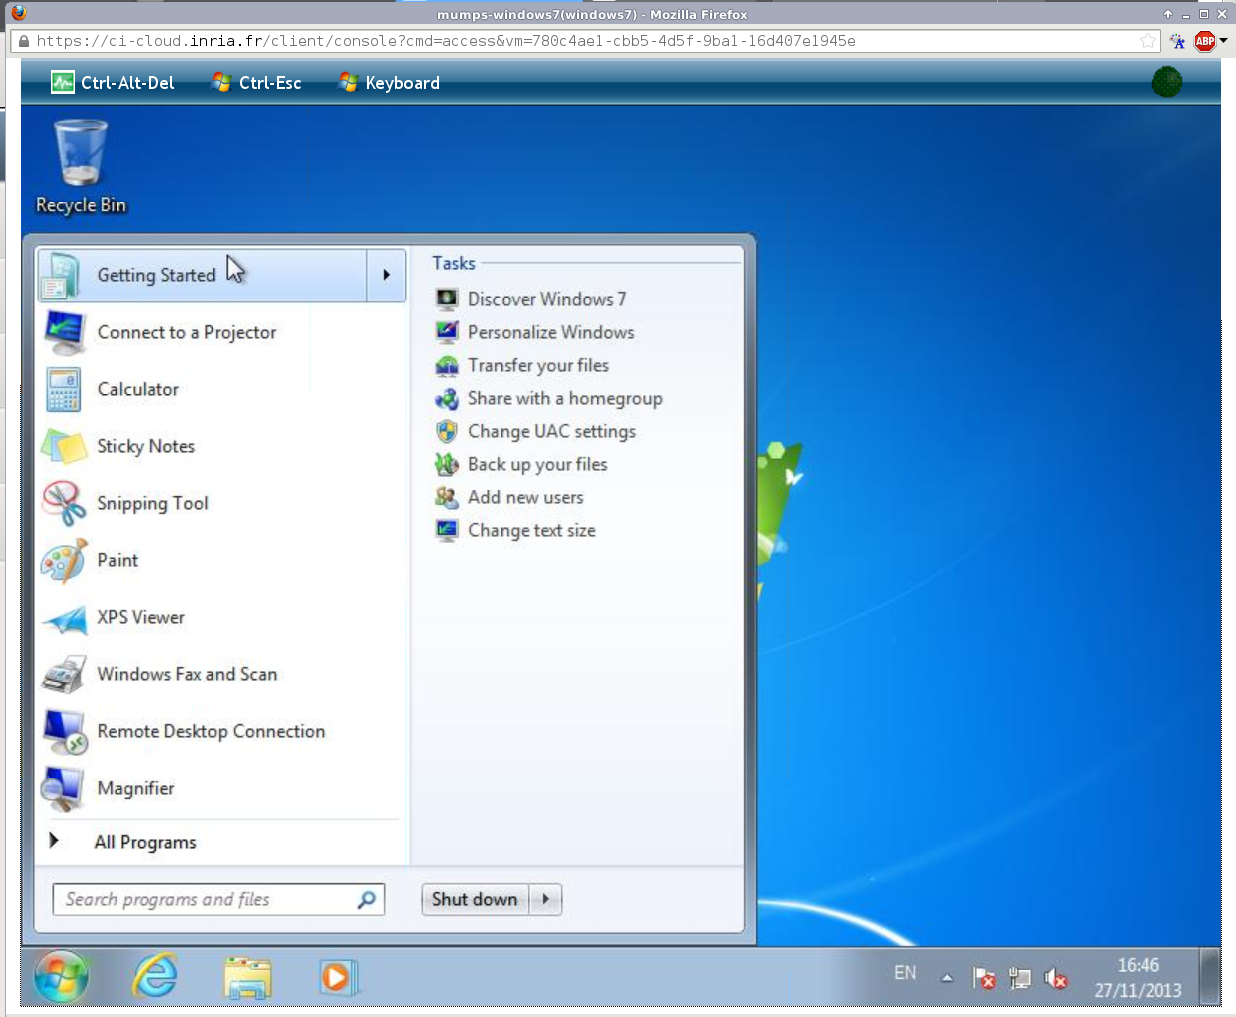
\includegraphics[width=.4\textwidth] {images/cloudstack-windows-desktop.png}};
 \path[->, thick, color=red] (select.south) edge [bend left] (windows_desktop.east);

\end{tikzpicture}
\end{frame}



% Retour d'expérience
% *******************
\inriaswitchcolors{green}
\section{Un retour d'expérience}
\frame{\tableofcontents[currentsection]
  \note{Vous avez besoin d'intégration continue\\}
  \note{Exemple mon expérience personnelle}
}

\subsection{Contexte de développement}
\tocsubsection{\note{Justifié de le faire pour moi, vous reconnaître sur certains points}}

\subsubsection{FIT Equipex - Future Internet of Things}
\begin{frame}{\subsubsecname} %{\subsecname}
  \note[item]{Equipex: 'equipement excellence' projet FR}
  \note[item]{Future Internet of Thing.}
  \note[item]{plusieurs plateformes}
  \note[item]{Durée de 10 ans}
  \note[item]{}
  \note[item]{IOT-LAB - description slide suivant}

  \begin{center}
    \begin{tabular}{ l l }
      
\includegraphics[width=0.2\textwidth]{images/logo_invest_avenir} &
      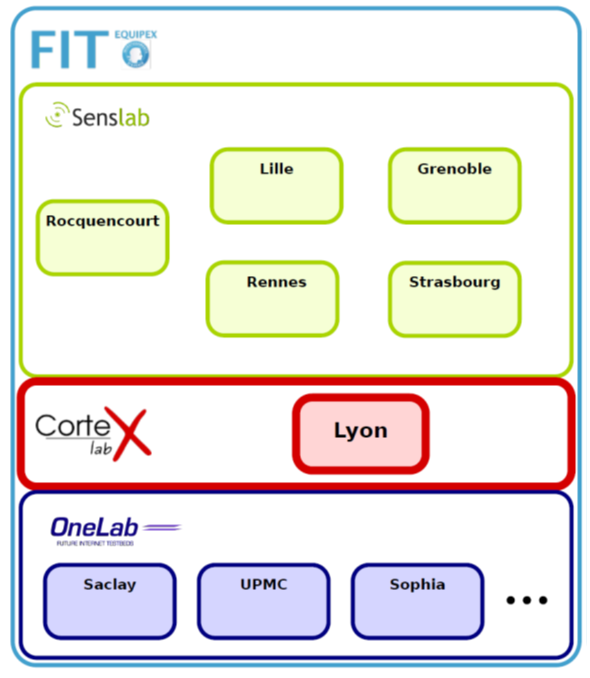
\includegraphics[width=0.5\textwidth]{images/fit_equipex} \\
    \end{tabular}
  \end{center}
\end{frame}


\subsubsection{Plateforme de réseau de capteurs: FIT IoT-LAB}
\begin{frame}{\subsubsecname} %{\subsecname}
  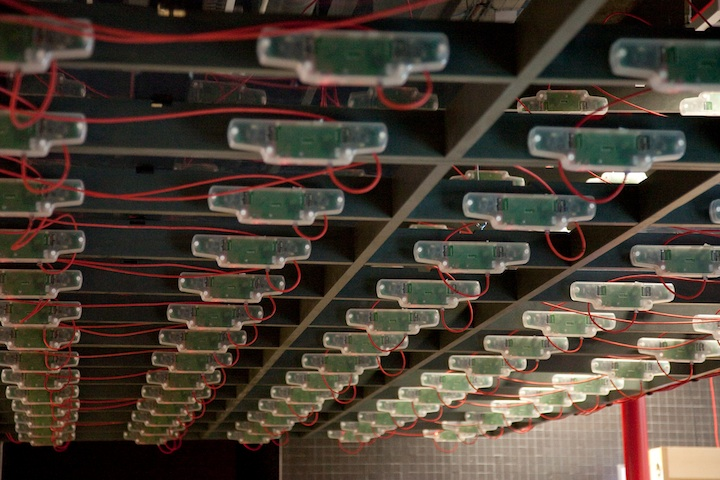
\includegraphics[width=\textwidth]{images/senslab_nodes}
  \note[item]{IoT-LAB: réseaux de capteurs 'objets connectés', 3000}
  \note[item]{Objets qui communiquent courte distance, et joignable depuis l'internet}
  \note[item]{Mis à disposition des chercheurs}
  \note[item]{2 générations de capteurs}
\end{frame}

\begin{frame}{\subsubsecname} %{\subsecname}
  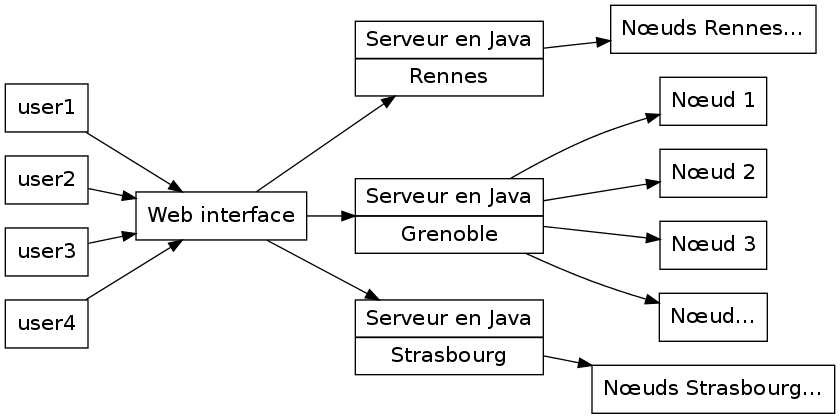
\includegraphics[width=\textwidth]{images/fit_architecture}
  \note{Exemple d'un chercheur voulant expérimenter sur les réseaux de capteurs}
  \note[item]{Se connecter sur l'interface web}
  \note[item]{Réserver un grand nombre de nœuds capteurs (3k dispos)}
  \note[item]{Déployer des programmes dessus}
  \note[item]{Interragir avec eux par connection série}
  \note[item]{Monitorer leur fonctionnement, conso, radio}
\end{frame}


\subsubsection{Un nœud capteur IoT-LAB}
\begin{frame}{\subsubsecname} %{\subsecname}
  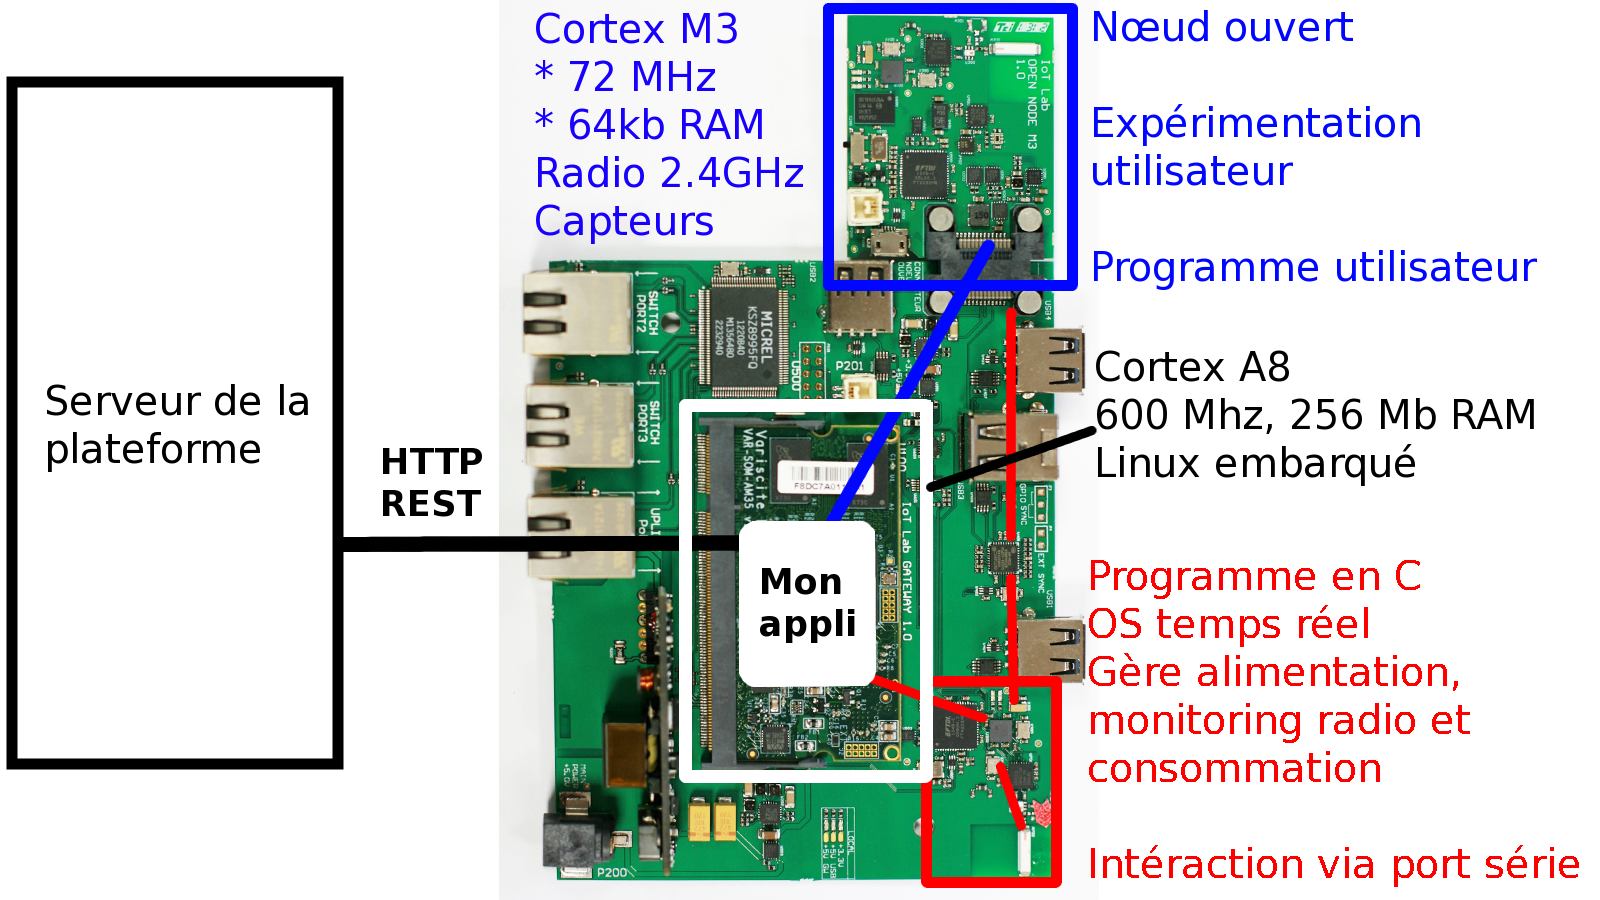
\includegraphics[width=\textwidth]{images/gateway_m3_annote}
\end{frame}

\subsubsection{Contexte de l'application}
\begin{frame}{\subsubsecname} %{\subsecname}
  \begin{itemize}
    \item Python + C (+ outils compilés externes)
    \item Application mise en production (QoS)
    \item Exécution sur une carte ARM avec Linux embarqué (perf...)
    \item Intéractions extérieures
    \item multithread, multiprocess
  \end{itemize}
\end{frame}


\subsubsection{Pourquoi avoir mis place de l'intégration continue}
\begin{frame}{\subsubsecname} %{\subsecname}
  \begin{itemize}
    \item Sources d'erreurs non déterministes
      \note[item]{Dépendance à du matériel}
      \note[item]{Dépendance à des programmes qui ne sont pas sur la même machine}
      \note[item]{Multithread et multiprocess}
      \note[item]{}
    \item Logiciel final doit être fiable
      \note[item]{service 24/7}
      \note[item]{Coût d'un bug: Debug, mise à jour}
      \note[item]{Large échelle, proba d'apparition d'un bug}
      \note[item]{}
    \item J'avais envie d'essayer
    \item La chose qui m'a décidée…
  \end{itemize}
\end{frame}

\subsubsection{J'avais besoin d'un seul test}
\begin{frame}[fragile]{\subsubsecname} %{\subsecname}
  \setbeamercovered{transparent}

  \begin{verbatim}

  def thread_redirection(self):
      while not self.stop:
          self.proc = subprocess.Popen(['socat', ...)
          self.proc.wait()
          if 0 != self.proc.returncode:
              # Gestion de l'erreur

  def stop(self):
      while self.is_alive():
          self.proc.terminate()
          time.sleep(0.1)

  \end{verbatim}

  \onslide <2-> Test sur carte: '\texttt{ImportError: No module named arpgarse}'


\end{frame}



\subsection{Outils mis en place}
\tocsubsection{
  \note[item]{Juste une overview, un exemple}
  \note[item]{Quelques possibilité et contraintes}
  \note[item]{En utilisant ci.inria.fr}
}

\subsubsection{Présentation des outils}
\begin{frame}{Outils mis en place}

  Gestionnaire de versions: \texttt{git} \\ ~ \\

  \begin{tabular}{ l | l l | p{3.5cm} }
    Language         & \texttt{Python}     & \texttt{C}    & Exploitation dans Jenkins \\ \hline
    Script de build  & \texttt{setuptools} & \texttt{Make} & Bash~shell, \texttt{EnvInject} \texttt{virtualenv}\\
    Compilation      & ~                   & \texttt{gcc}  & ~ \\
    Tests            & \texttt{nose}, \texttt{unittest}, \texttt{mock}
                     & \texttt{gtest} \texttt{(C++)}
                     & Junit, Chuck Norris\\
    Couverture       & \texttt{nose-xcover}
                     & \texttt{gcov}, \texttt{gcovr}
                     & Cobertura \\
   Qualité de code  & \texttt{pylint}, \texttt{pep8} & ~  & Violations \\
    ~ & ~  & ~ & \\
    Lignes de code   &  $3000$        &  $1500$  &  $0$  \\
    Lignes de tests  &  $1600 + 400$  &  $1300$  &  $0$  \\
% 1600 tests U + 400 tests intégration
    Lignes de build  &  $300$         &  $170$   &  $50$ \\

    \note[item]{Gestion de version, partagée avec d'autres projets}
    \note[item]{Correspondance entre outils mis en place et Jenkins, \textbf{fichiers générés}}
    \note[item]{Types d'outils les uns après les autres}
    \note[item]{Pylint remplace compilation python}
    \note[item]{}
    \note[item]{1600 tests U + 400 tests intégration}
    \note[item]{SQLite 3.8 == 1084 * plus de tests que de code 84k source (hors blank et commentaires)}
  \end{tabular}
\end{frame}


\subsubsection{Jenkins}
\begin{frame}{Présentation outils}{Jenkins}
  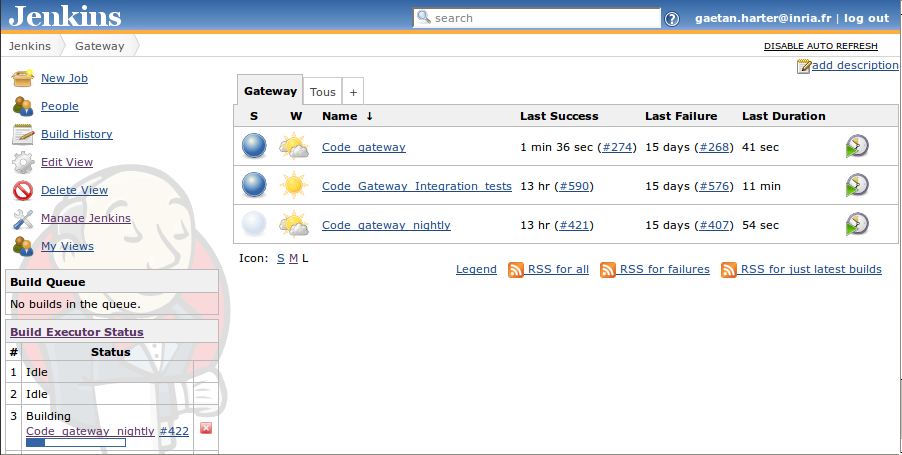
\includegraphics[width=\linewidth]{images/jenkins}
  \note[item]{2 types}
  \note[item]{Sur carte cible \textbf{Thales}}
  \note[item]{Lancement des tests, à la main et toute les nuits}
\end{frame}

\begin{frame}{Configuration d'un build}{Jenkins}
  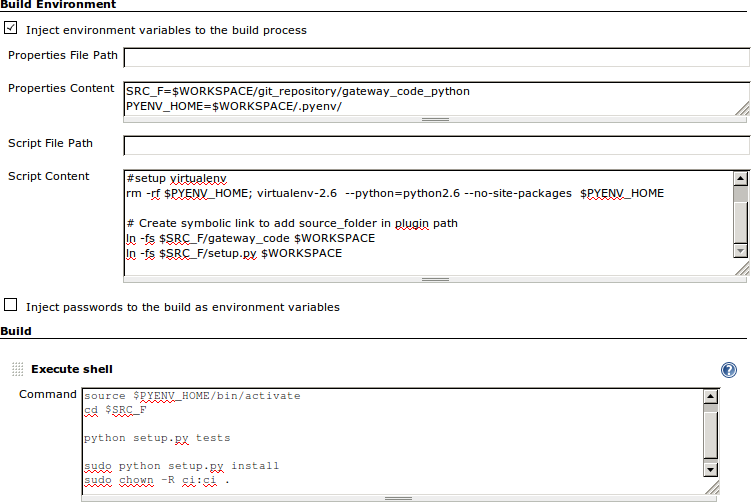
\includegraphics[width=\linewidth]{images/build_configuration}
\end{frame}


\begin{frame}{Cobertura}{Jenkins}
        % Pour moi, l'outil le plus important (après Chuck Norris forcément)
  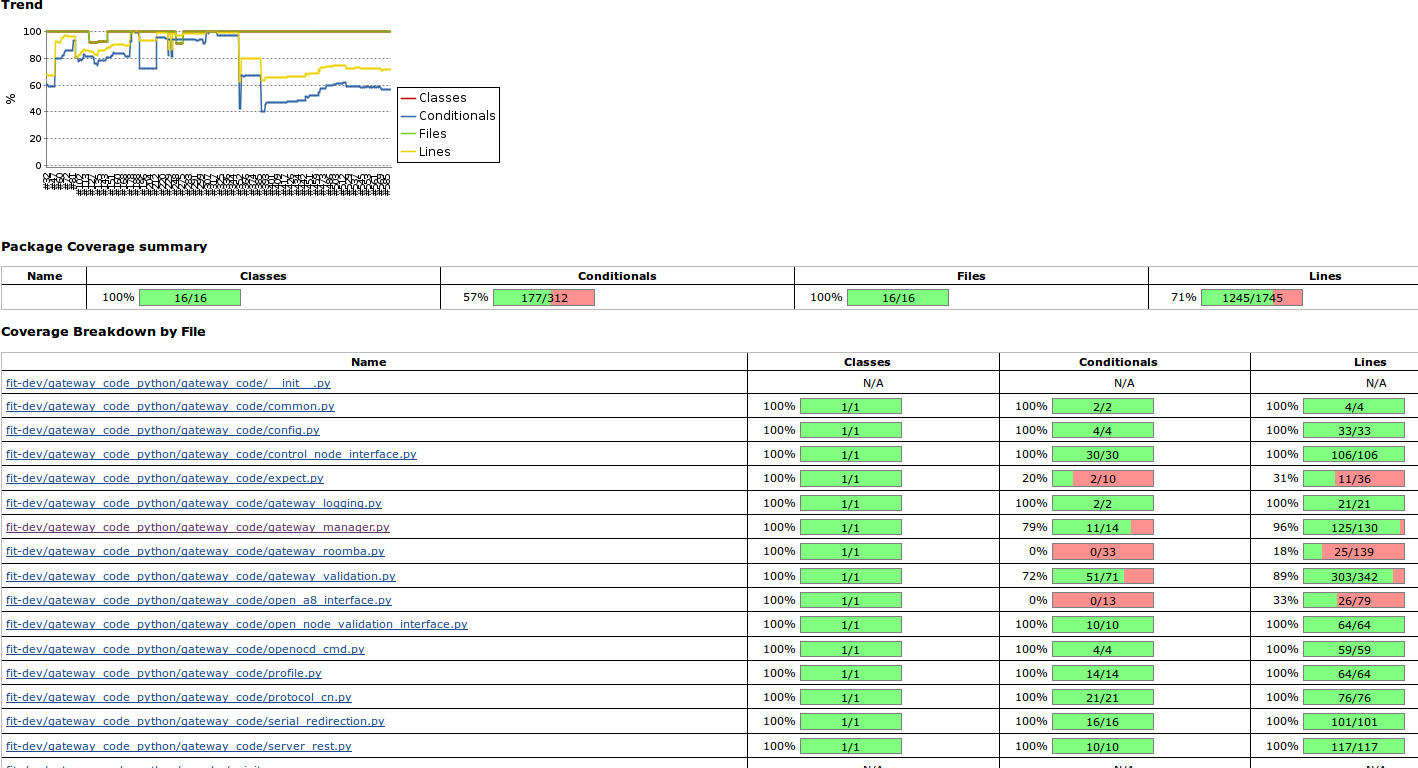
\includegraphics[width=\linewidth]{images/cobertura}\\
\end{frame}
\begin{frame}{Junit - Violations}{Jenkins}
  \begin{center}
        % Juste pour montrer
    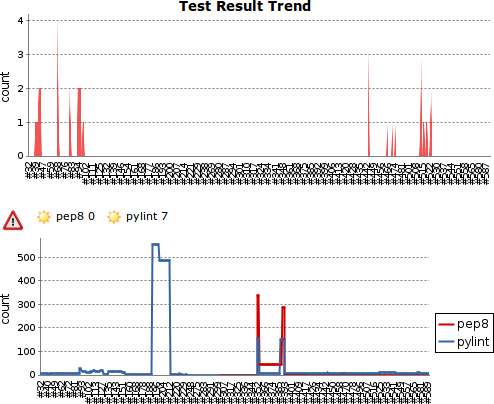
\includegraphics[height=0.8\textheight]{images/junit_violations}\\
  \end{center}
\end{frame}
\begin{frame}{Chuck Norris}{Jenkins}
  % Le plus important des plugins
  \begin{center}
    \begin{tabular}{ l |l }
      Build KO & Build OK \\ \hline
        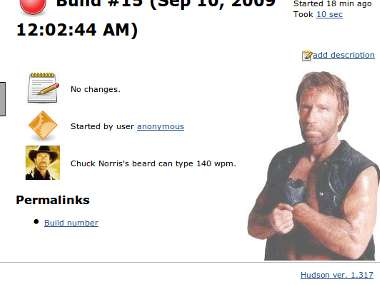
\includegraphics[height=4cm]{images/chuck_full} &
      
\includegraphics[height=4cm]{images/chuck_happy}
        %
\includegraphics[height=4cm]{images/chuck_angry}
      \\
    \end{tabular}
  \end{center}
  Chuck Norris Facts:
  \begin{itemize}
    \item Chuck Norris can unit test an entire application with a single assert.
    \item Chuck Norris can divide by zero.
    \item ...
  \end{itemize}
\end{frame}




\subsection{Bilan}
\tocsubsection


\subsubsection{Développement logiciel}
\begin{frame}{\subsubsecname}{\subsecname}
  \note{GROS SLIDE}

  \begin{itemize}
    \item Mise en place d'un script de \texttt{build}
      \note[item]{Procédure de test, même 1 seul test}
      \note[item]{Procédure simple dans un script}
      \note[item]{}
    \item Tests nombreux et lancés en continu
      \note[item]{Gestion des cas d'erreurs}
      \note[item]{Détection de problèmes tot (perf réimplèm en C}
      \note[item]{simplification de l'implem}
      \note[item]{dev itératif}
      \note[item]{Detection d'erreurs rares}
      \note[item]{}
    \item Couverture de code
      \note[item]{Même si $<100\%$, savoir ce qui est 'validé' et ce qui ne l'est pas}
    \item Qualité de code
      \note[item]{Python: Remplace la phase de compilation (vérification syntaxique)}
      \note[item]{Détection statique d'erreurs}
      \note[item]{Standardisation de la mise en forme, lisibilité (PEP8)}
      \note[item]{}
  \end{itemize}
  Maîtrise et confiance dans le logiciel développé
\end{frame}

\subsubsection{Personnel}
\begin{frame}{\subsubsecname}{\subsecname}
  \begin{itemize}
    \item Découverte de beaucoup d'outils
    \item Maîtrise des languages et leur écosystème
    \item Confort dans le développement
    \item Retours positifs après premières utilisations
    \item J'aimerai maintenant pouvoir l'appliquer à d'autres choses
  \end{itemize}
  \note[item]{Rassurant}
  \note[item]{Je peux tester!}
\end{frame}

\subsubsection{Voies d'amélioration}
\begin{frame}{\subsubsecname}{\subsecname}
  \begin{itemize}
    \item Passer les configurations Jenkins dans des scripts versionnés
    \item Grouper Python et C dans le build python
    \item Inclusion d'autres développeurs
    \item 100\% de couverture de code
  \end{itemize}
\end{frame}


\begin{frame}{The End}
  Merci d'avoir écouté.
\end{frame}


\end{document}
